\chapter{Die Realisierung}
\label{cha:Realisierung}
Folgendes Kapitel befasst sich mit der Implementierung, der im Kapitel \ref{cha:Lösungskonzept} vorgestellten Spezifikation des Vorlagenmanagements. Die Implementierung wurde in \emph{Java 8} mit dem \emph{Buildtool Maven} realisiert, wobei die Implementierungen in der folgenden Projektstruktur organisiert wurden.
\newline
\dirtree{%
.1 mailing.
.2 module.
.3 template.
.4 cdi.
.4 jsf.
.4 model.
.5 json.
.4 logic.
.5 api.
.5 impl.
.3 integration.
.4 clevercure-web.
.2 testsuite.
.3 cdi.
.2 demo.
.3 web.
.2 data.
.3 api.
.3 impl.
}
\ \newline
Das Wurzelprojekt \emph{mailing} organisiert alle Abhängigkeiten für die Unterprojekte sowie die gemeinsame \emph{Build}-Konfiguration, die auf alle konkreten Projekte angewendet werden kann. Ebenfalls enthält es die Metadaten wie die EntwicklerInnen, die an diesem Projekt mitwirken. Die Unterprojekte, die ebenfalls \emph{Paren}-Projekte bündeln ihre Unterprojekte und organisieren keine Abhängigkeiten und definieren keine Metadaten. Die gesamte Organisation findet im \emph{Paren}-Projekt \emph{mailing} statt. Diese Projektstruktur wurde gewählt, da in diesem Projekt in weitere Folge auch die Implementierungen der anderen benötigten Softwarekomponenten des \emph{Mail-Service} beinhalten wird. Die konkreten Artefakte wurden jeweils in ein Artefakt \emph{*-api} und \emph{*-impl} aufgeteilt, somit sind die Schnittstellen vollständig getrennt von der Implementierung.
\newline
\newline
Die folgenden Artefakte resultieren aus dieser Projektstruktur, wobei nur die konkreten Artefakte und nicht die \emph{Parent}-Artefakte angeführt sind.
\begin{itemize}
	\item\emph{\textbf{mailing-module-template-logic-api}} ist das Artefakt, das die Spezifikation des Vorlagenmanagement enthält.
	\item\emph{\textbf{mailing-module-template-logic-impl}} ist das Artefakt, das die Implementierung der Spezifikation des Vorlagenmanagements enthält.
	\item\emph{\textbf{mailing-module-template-cdi}} ist das Artefakt, das die Implementierung für die Integration in einen \emph{CDI-Container} enthält.
	\item\emph{\textbf{mailing-module-template-jsf}} ist das Artefakt, das die Implementierung für die Integartion in \emph{JSF} enthält.
	\item\emph{\textbf{mailing-module-template-model-json}} ist das Artefakt, das die Implementierung der \emph{JSON}-Spezifikation enthält.
	\item\emph{\textbf{mailing-module-integartion-clevercure-web}} ist das Artefakt, das die Implementierung der Integration für die Anwendung \emph{CleverWeb} enthält.
	\item\emph{\textbf{mailing-data-api}} ist das Artefakt, dass die Spezifikation der \emph{Services} enthält.
	\item\emph{\textbf{mailing-data-impl}} ist das Artefakt, das die Implementierung der \emph{Service}-Spezifikation enthält.
	\item\emph{\textbf{mailing-testsuite-cdi}} ist das Artefakt, das die Basis aller Tests, die in einem \emph{CDI-Container} lauffähig sein sollen darstellt.
	\item\emph{\textbf{mailing-demo-web}} ist das Artefakt, das die Demowebanwendung darstellt.
\end{itemize} 
\ \newline


\section{Die Implementierung der Spezifikationen}
Der folgende Abschnitt behandelt die Implementierungen der im Kapitel \ref{cha:Lösungskonzept} vorgestellten Spezifikation.

\subsection{Die Implementierung für \emph{CKEditor}}
\emph{CKEditor} ist ein \emph{Javascript} basierter mit dem die Vorlagen bearbeitet werden können. Wie in \ref{sec:sub-typescript-javascript} vorgegeben wird ein \emph{Plugin} benötigt, dass innerhalb des \emph{CKEDitor} die Variablen verwalten kann. Diese \emph{Plugin} wurde in \emph{Typescript} implementiert, da hier Typsicherheit vorhanden ist im Gegenzug zu Javascript das nicht typsicher ist. Die Implementierung des \emph{Plugins} in \emph{Typescript} war möglich, da für den \emph{CKEditor} Typinformationen für \emph{Typescript} vom dem \emph{Open-Source} Projekt \emph{DefinitelyTyped} bereitgestellt wird. \emph{Typescript} benötigt Typinformationen für \emph{Javascript} Quelltext, damit die Typsicherheit in \emph{Typescript} gewährleistet werden kann. Würden keine Typinformationen zur Verfügung stehen, hätte man sie selber implementieren müssen. 
\newline
\newline
Der Quelltext befindet sich zurzeit im Projekt \emph{mailing-demo-web}, da die Verwendung eines \emph{Web-Fragment} das Problem mit sich bringt, dass während der Entwicklung die Ressourcen nicht automatisch nachgeladen werden können, was die Entwicklung sehr erschwert. Da es sich aber nur um zwei Quelltexte handelt, die einfach verschoben werden können, stellt das kein Problem dar.
 
\subsubsection{Das \emph{CKEDitor-Plugin} in Typescript}
Da das Variablenmanagement unabhängig vom verwendeten \emph{CKEditor} ist, wurde die Verwaltung der Variablen in einem eigenen \emph{Javascript} Modul \emph{cc.variables} zusammengefasst. Das \emph{CKEditor Plugin} wurde im \emph{Javascript} Modul \emph{cc.ckeditor.plugins} zusammengefasst. Das Variablenmanagement in \emph{Typescript} ist verantwortlich für die \emph{Browser} seitige Registrierung der Variablen und stellt Hilfsmethoden zur Verfügung zur Verfügung, mit denen Variablen in der \emph{Registry} gefunden und konvertiert werden können. Folgendes Beispiel soll illustrieren wie eine Variable konvertiert werden kann.
\begin{JsCode}[numbers=none]
// Signature of the converter function
public convertVariables(converter:(item:VariableMapping) => any 
                        = (item:VariableMapping)=> item):any[]

// Convert to the variable's set displayName
variablesHandler.convertVariables(
	function (variable) {
		return variable.displayName;
	}
)                        
\end{JsCode}
Die Funktion \emph{convertVariables} definiert den Formalparameter \emph{converter} als eine sogenannte \emph{Arrow}-Funktion, die einer \emph{Lambda}-Funktion in \emph{Java} ähnelt. Mit der \emph{Arrow}-Funktion wird die Signatur der Funktion für die Konvertierung vorgegeben. Ebenfalls wird für den Formalparameter \emph{converter} eine Standardimplementierung definiert, die verwendet wird, sollte der Formalparameter \emph{converter} bei Aktivierung der Funktion \emph{convertVariables} nicht gesetzt sein. Der Typ \emph{any[]} ist vergleichbar mit dem Datentyp \emph{var} aus \emph{.NET} und gibt an das jeder Datentyp als Typ des zurückgelieferten \emph{Arrays} erlaubt ist.
\newline
\newline
Das \emph{CKEditor Plugin} ist für die Integration der Variablen in den \emph{Editor} verantwortlich, wobei die zur Verfügung stehenden über einen Dialog ausgewählt werden können. Ausgewählte variablen werden an die aktuelle Position des Cursors im \emph{Editor} in Form einer \emph{HTML Tags} platziert.
\begin{figure}[h]
\centering
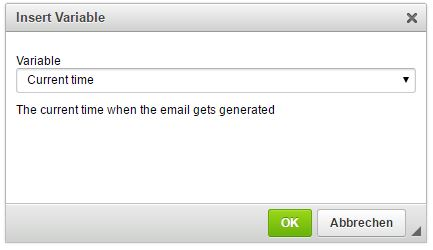
\includegraphics[scale=1]{ckeditor-dialog-insert-variable}
\caption{\emph{CKEditor} Dialog für die Variablenauswahl}
\label{fig:clevermail-rest-tcc}
\end{figure}

\subsubsection{Die Variablenrepräsentation in JSON}


\subsection{Die Implementierungen für CDI}

\subsubsection{Die Vorlagen-\emph{Management CDI-Extension}}

\subsubsection{Der Vorlagen-\emph{Management CDI-Producer}}

\subsubsection{Die Vorlagen-\emph{Management CDI-Utility}}


\subsection{Die Implementierungen für JSF}

\subsubsection{Der Vorlagen \emph{FacesConverter}}

\subsubsection{Die \emph{Primefaces-Extension} für den \emph{CKEditor}}


\section{Die Vorlagen-\emph{Management} Beispielanwendung}
\subsection{Die Verwendung in einem \emph{Business}-Service}
\subsection{Die Verwendung in der \emph{Web}-Oberfläche}